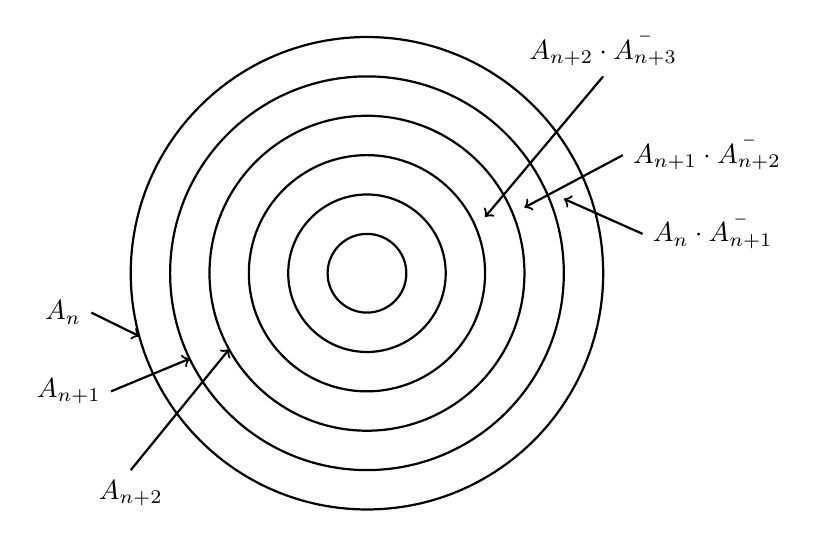
\begin{tikzpicture}[scale = 0.5]
  \foreach \d in {1, ..., 6} {
    \draw[thick] (0, 0) circle (\d cm);
  }
  \draw[->, thick] (-7, -1) -- (-5.78, -1.6)
    node[pos = 0, left] {\(A_n\)};
  \draw[->, thick] (-6.5, -3) -- (-4.5, -2.17)
    node[pos = 0, left] {\(A_{n + 1}\)};
  \draw[->, thick] (-6, -5) -- (-3.5, -1.93)
    node[pos = 0, below] {\(A_{n + 2}\)};

  \draw[->, thick] (7, 1) -- (5, 1.89)
    node[pos = 0, right] {\(A_n \cdot \bar{A_{n + 1}}\)};
  \draw[->, thick] (6.5, 3) -- (4, 1.67)
  node[pos = 0, right] {\(A_{n + 1} \cdot \bar{A_{n + 2}}\)};
  \draw[->, thick] (6, 5) -- (3, 1.43)
  node[pos = 0, above] {\(A_{n + 2} \cdot \bar{A_{n + 3}}\)};

\end{tikzpicture}